\documentclass[aspectratio=169]{beamer}
\mode<presentation>
{
  \usetheme{metropolis}      % or try Darmstadt, Madrid, Warsaw, ...
  \usecolortheme{default} % or try albatross, beaver, crane, ...
  \usefonttheme{structurebold}  % or try serif, structurebold, ...
  \setbeamercolor{background canvas}{bg=white}
  \setbeamertemplate{navigation symbols}{}
  \setbeamertemplate{bibliography item}{\insertbiblabel}
  %\setbeamertemplate{caption}[numbered]
} 
\usepackage[english]{babel}
\usepackage[utf8x]{inputenc}
\usepackage{listings}             % Include the listings-package
\hypersetup{
    colorlinks = true,
    linkcolor = {black},
    urlcolor = {blue}
}

\usepackage{animate}
\usepackage{listings}
\usepackage{bm}

\DeclareMathOperator*{\argmin}{arg\,min}

\title[Semi-supervised learning via Deep Denoising Autoencoders]{Semi-supervised learning via Deep Denoising Autoencoders}
\subtitle{Autoencoders in TensorFlow}
\institute{University of Modena and Reggio Emilia}
\author{Angelo Porrello, Davide Abati}

\def\thisframelogos{}

\newcommand{\framelogo}[1]{\def\thisframelogos{#1}}

\addtobeamertemplate{frametitle}{}{%
\begin{tikzpicture}[remember picture,overlay]
\node[anchor=north east] at (current page.north east) {%
    \foreach \img in \thisframelogos {%
        %\hspace{.5ex}%
        \includegraphics[height=3.5ex]{\img}%
    }%
};
\end{tikzpicture}}

\begin{document}

\framelogo{img/template/logo_unimore_white.png}

\bgroup
\renewcommand{\insertframenumber}{}
\begin{frame}[noframenumbering]
  \titlepage
\end{frame}
\egroup
\begin{frame}{Agenda}
  \tableofcontents
\end{frame}


%%%%%%%%%%%%%%%%%%%%%%%%%%%%%%%%%%%%%%%%%%%%%%%%%%%%%%%%%%%%%%%%%%

\section{Autoencoders}

\begin{frame}{Autoencoders}
An \textbf{autoencoder} is a feed-forward neural network that is trained to attempt to copy its input to its output.
The network may be viewed as consisting of two parts: an encoder function
$h=f(x)$ and a decoder that produces a reconstruction $r=g(h)$.
\vspace{0.4cm}
\begin{figure}
    \centering
	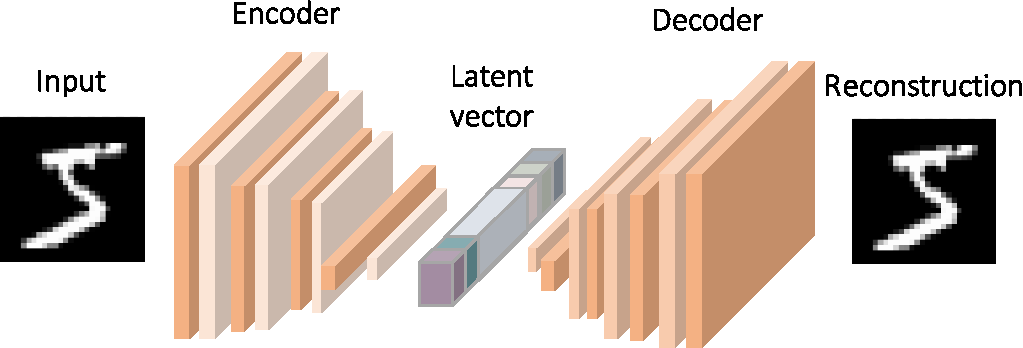
\includegraphics[width=0.80\textwidth]{img/autoencoder/naive.pdf}
\end{figure}
\end{frame}

\begin{frame}{Autoencoders}
The learning process plans to minimize $\mathcal{L}(g(f(x))$ where $\mathcal{L}$ is a loss function penalizing $g(f(x))$ for being dissimilar from $x$, e.g. the Mean Square Error (MSE).
\begin{equation}
    \mathcal{L}(g(f(x)) = \left\| x - g(f(x) \right\|_{2}
\end{equation}
\begin{figure}
    \centering
	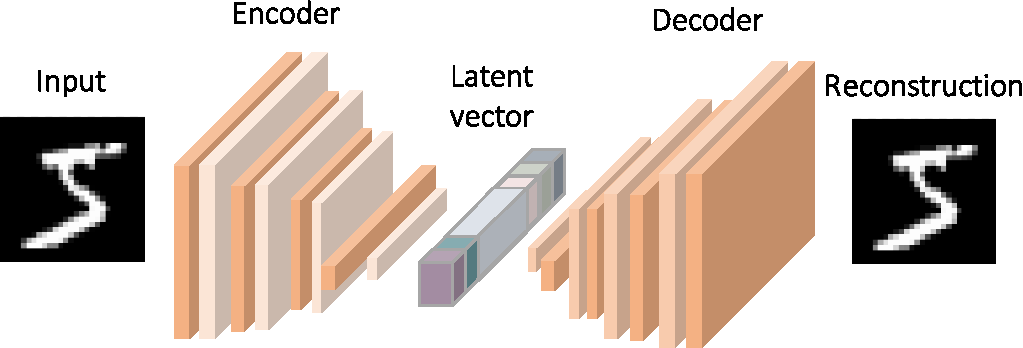
\includegraphics[width=0.80\textwidth]{img/autoencoder/naive.pdf}
\end{figure}
\end{frame}

\begin{frame}{Autoencoders}
The \textbf{aim} is to induce in h useful properties and the most salient features of the training data.
For instance, \textbf{lower dimensional representations} attempt to compress as much information about x in a smaller representation.
\vspace{0.4cm}
\begin{figure}
    \centering
	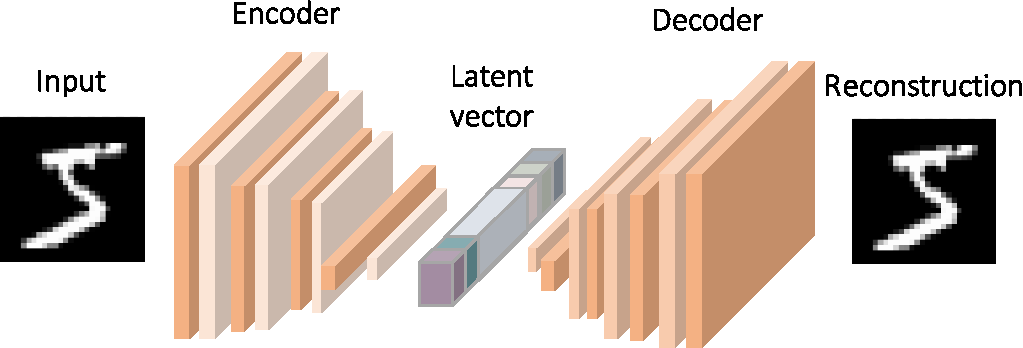
\includegraphics[width=0.80\textwidth]{img/autoencoder/naive.pdf}
\end{figure}
\end{frame}

\begin{frame}{Denoising Autoencoders (DAE)}
In order to avoid learning the identity function, autoencoders are restricted in ways that allow them to copy only \textbf{approximately}. To capture more robust features in the hidden layer, a denoising autoencoder is trained to reconstruct the input x from a \textbf{corrupted} version $\tilde{x}$ of it.
\vspace{0.4cm}
\begin{figure}
    \centering
	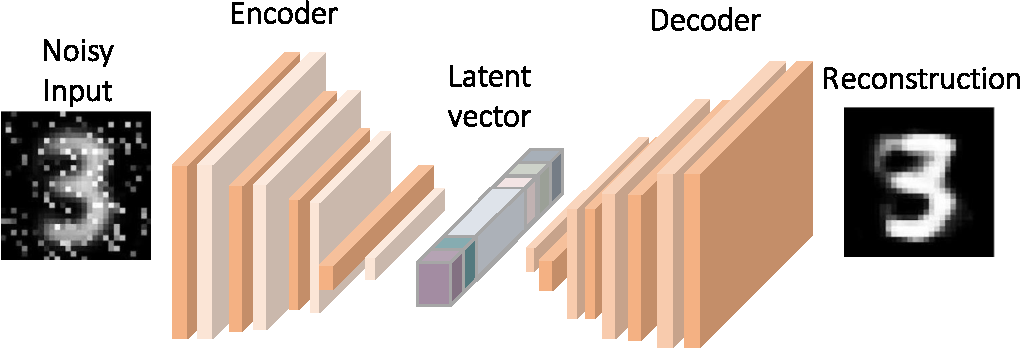
\includegraphics[width=0.80\textwidth]{img/autoencoder/denoising.pdf}
\end{figure}
\end{frame}

\begin{frame}{Denoising Autoencoders (DAE)}
The corrupted input $\tilde{x}$ can be obtained applying on x some form of noise e.g additive white gaussian noise or dropout. Then, the DAE must undo this corruption rather than simply copying their input.
\begin{equation}
    \mathcal{L}(g(f(x)) = \left\| x - g(f(\tilde{x}) \right\|_{2} \quad \tilde{x} \sim \mathcal{N}(x,\,\sigma^{2}\text{I})\
\end{equation}
\begin{figure}
    \centering
	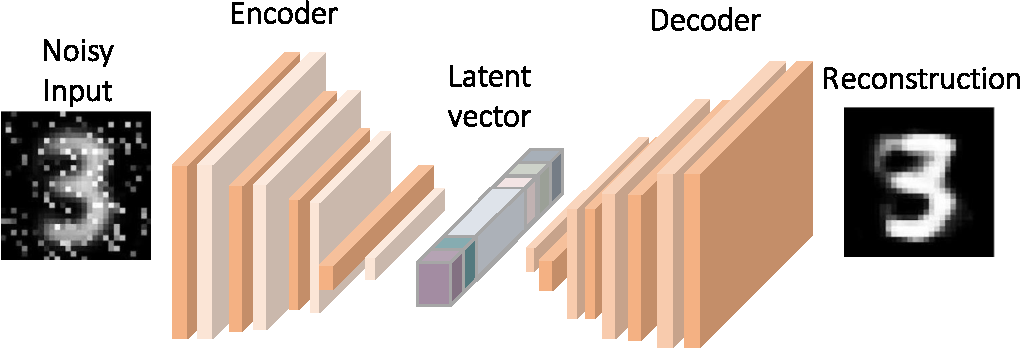
\includegraphics[width=0.80\textwidth]{img/autoencoder/denoising.pdf}
\end{figure}
\end{frame}

%%%%%%%%%%%%%%%%%%%%%%%%%%%%%%%%%%%%%%%%%%%%%%%%%%%%%%%%%%%%%%%%%%

\section{Semi-supervised learning}

\begin{frame}{Semi-supervised learning}
\textbf{Problem:} Deeper models lead to more parameters, which implicates the requirement for a high number of training data in order to avoid overfitting.\\
\vspace{0.4cm}
\textbf{Semi-supervised learning} regards a class of machine learning techniques combining both labeled and unlabeled data.\\
\vspace{0.4cm}
\textbf{Goal:} taking advantage of a large amount of \textbf{unlabeled data} to learn a suitable representation, and then exploit it for training a new classifier, the latter leveraging just few labeled data. 
\end{frame}
\begin{frame}{Semi-supervised learning with Autoencoders}
\begin{tabular}{c}
	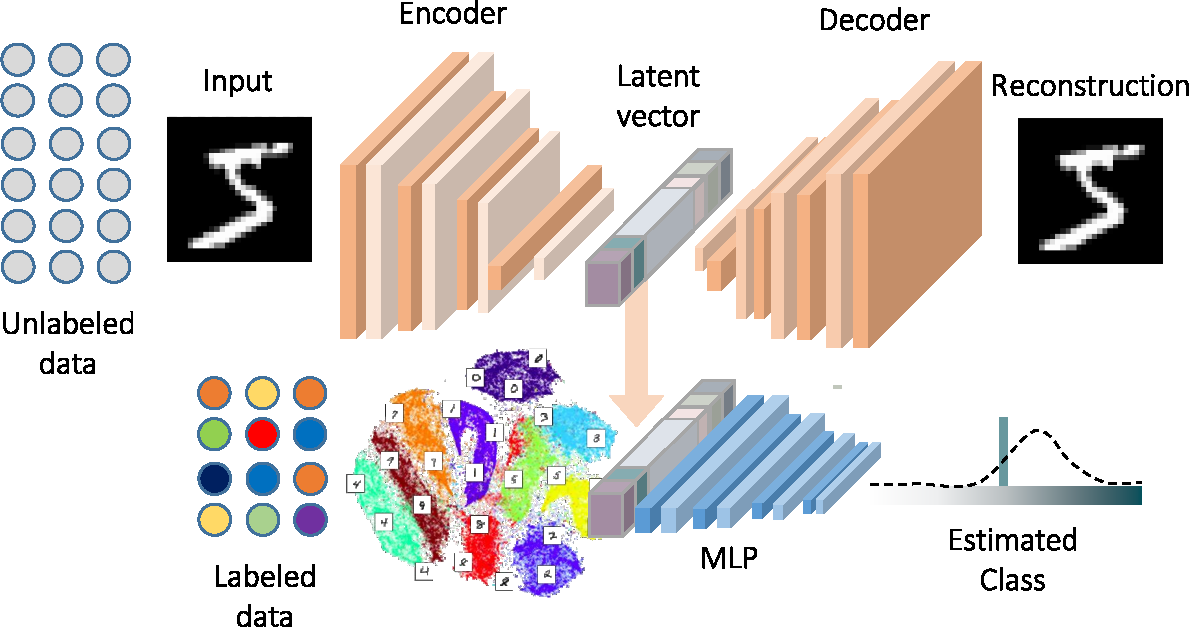
\includegraphics[width=0.95\textwidth]{img/autoencoder/semi.pdf}
\end{tabular}
\end{frame}

%%%%%%%%%%%%%%%%%%%%%%%%%%%%%%%%%%%%%%%%%%%%%%%%%%%%%%%%%%%%%%%%%%

\section{Semi-supervised learning on MNIST}

\begin{frame}{Semi-supervised learning on MNIST}
\begin{columns}
\begin{column}{0.5\textwidth}
\begin{enumerate}
    \item Given the MNIST training set, discard the labels and train a denoising autoencoder on it. As a starting point, provide a DAE with just dense layers, batch normalization and the non-linearity you prefer. 
\end{enumerate}
\vspace{0.4cm}
Once it has been trained, extract bottleneck activations for both training and test set.
\end{column}
\begin{column}{0.5\textwidth}  %%<--- here
    \begin{center}
	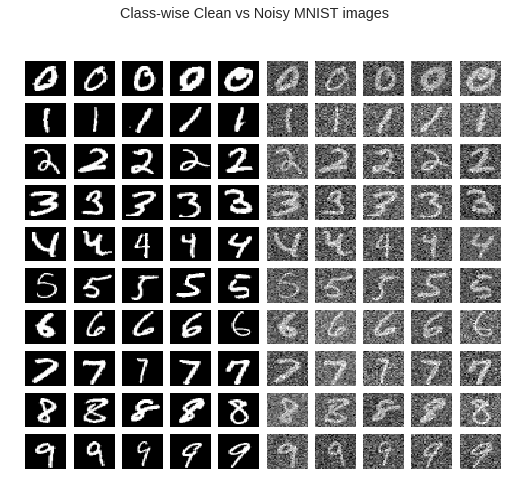
\includegraphics[width=1.0\textwidth]{img/autoencoder/mnist_noisy.png}
     \end{center}
\end{column}
\end{columns}
\end{frame}

\begin{frame}{Semi-supervised learning on MNIST}
\begin{figure}
    \centering
	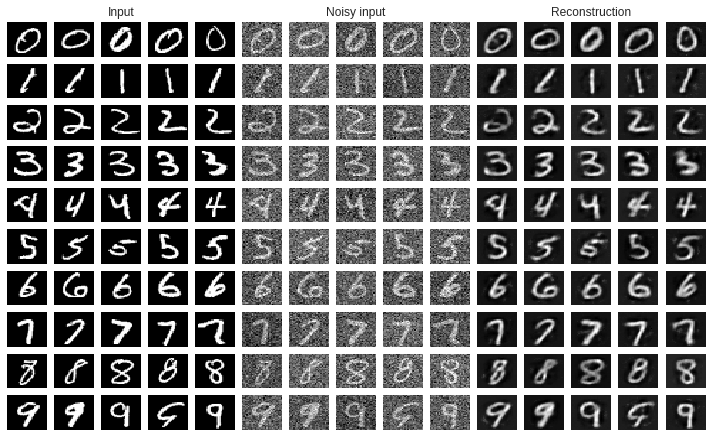
\includegraphics[height=0.90\textheight]{img/autoencoder/reconstructions.png}
\end{figure}
\end{frame}

\begin{frame}{Semi-supervised learning on MNIST}
\begin{enumerate}
    \setcounter{enumi}{1}
    \item To emulate a setting with few labeled samples, pick a small subset of the original and fully-labeled training set (e.g. comprising just 200 randomly drawn samples among the 60000 available).
\end{enumerate}
\begin{columns}
\begin{column}{0.4\textwidth}
\begin{enumerate}
    \setcounter{enumi}{2}
    \item Train a simple classifier (e.g. K-NN) from both the grayscale features and the hidden activations. 
    \item Compare the test set classification accuracies arising from the two strategies.
\end{enumerate}\end{column}
\begin{column}{0.6\textwidth}  %%<--- here
    \begin{center}
	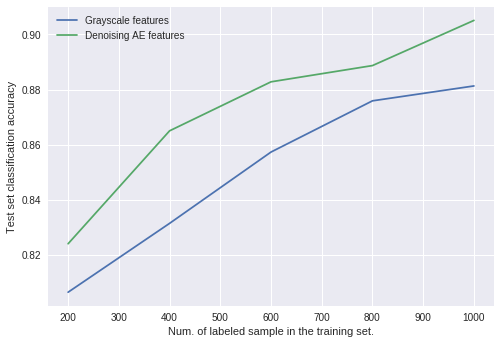
\includegraphics[width=0.90\textwidth]{img/autoencoder/accuracies.png}
     \end{center}
\end{column}
\end{columns}
\end{frame}

%%%%%%%%%%%%%%%%%%%%%%%%%%%%%%%%%%%%%%%%%%%%%%%%%%%%%%%%%%%%%%%%%%

\begin{frame}{Useful Functions}
To this purpose, you may find useful the following functions:
\begin{itemize}
\item \texttt{tf.cond}
\item \texttt{tf.random\_normal}
\item \texttt{tf.layers.batch\_normalization}
\item \texttt{tf.layers.dense}
\end{itemize}
Please refer to the docs to know the exact API.
\end{frame}

\begin{frame}{Optionally}
\begin{itemize}
\item Replace the dense layers with 2D-convolutions.
\item Compare the results w.r.t. a \textbf{naive} autoencoder (where the input has not been corrupted).
\item Compare the results w.r.t. a \textbf{sparse} autoencoder.
\item Conduct experiments on a more challenging dataset (e.g. CIFAR-10). 
\end{itemize}
\end{frame}

%%%%%%%%%%%%%%%%%%%%%%%%%%%%%%%%%%%%%%%%%%%%%%%%%%%%%%%%%%%%%%%%%%

\begin{frame}{\ }
\centering{
\Large{Good Luck!}
}
\end{frame}

%%%%%%%%%%%%%%%%%%%%%%%%%%%%%%%%%%%%%%%%%%%%%%%%%%%%%%%%%%%%%%%%%%
%%%%%%%%%%%%%%%%%%%%%%%%%%%%%%%%%%%%%%%%%%%%%%%%%%%%%%%%%%%%%%%%%%
%%%%%%%%%%%%%%%%%%%%%%%%%%%%%%%%%%%%%%%%%%%%%%%%%%%%%%%%%%%%%%%%%%

\end{document}